% Copyright 2004 by Till Tantau <tantau@users.sourceforge.net>.
%
% In principle, this file can be redistributed and/or modified under
% the terms of the GNU Public License, version 2.
%
% However, this file is supposed to be a template to be modified
% for your own needs. For this reason, if you use this file as a
% template and not specifically distribute it as part of a another
% package/program, I grant the extra permission to freely copy and
% modify this file as you see fit and even to delete this copyright
% notice. 

\documentclass{beamer}

\usepackage[T2A]{fontenc}           % кодировка
\usepackage[utf8]{inputenc}         % кодировка исходного текста
\usepackage[english,russian]{babel} % локализация и переносы
\usepackage{graphicx}  % Для вставки рисунков
\usepackage{listings}
\usepackage{color}
\usepackage[export]{adjustbox}
\usepackage{ragged2e}
\usepackage{tikz}
\usepackage{pgfplots}
\usepackage{tabularx}
\usepackage{multicol}
\usepackage{subcaption}


% There are many different themes available for Beamer. A comprehensive
% list with examples is given here:
% http://deic.uab.es/~iblanes/beamer_gallery/index_by_theme.html
% You can uncomment the themes below if you would like to use a different
% one:
%\usetheme{AnnArbor}
%\usetheme{Antibes}
%\usetheme{Bergen}
%\usetheme{Berkeley}
%\usetheme{Berlin}
%\usetheme{Boadilla}
%\usetheme{boxes}
%\usetheme{CambridgeUS}
%\usetheme{Copenhagen}
%\usetheme{Darmstadt}
\usetheme{default}
%\usetheme{Frankfurt}
%\usetheme{Goettingen}
%\usetheme{Hannover}
%\usetheme{Ilmenau}
%\usetheme{JuanLesPins}
%\usetheme{Luebeck}
%\usetheme{Madrid}
%\usetheme{Malmoe}
%\usetheme{Marburg}
%\usetheme{Montpellier}
%\usetheme{PaloAlto}
%\usetheme{Pittsburgh}
%\usetheme{Rochester}
%\usetheme{Singapore}
%\usetheme{Szeged}
%\usetheme{Warsaw}


\tikzset{>=latex}

\pgfkeys{
	mygrid/.is family,
	mygrid,
	width/.initial=2,
	height/.initial=2,
	step/.initial=1,
	color/.initial=black,
}
\newcommand\mygridset[1]{\pgfkeys{mygrid,#1}}
\newcommand\mygrid[1][]{
	\mygridset{#1,
		width/.get=\gridwidth,
		height/.get=\gridheight,
		step/.get=\gridstep,
		color/.get=\gridcolor
	}
	
	\draw [step=\gridstep, thick,\gridcolor]
	(0,0) grid (\gridwidth,\gridheight);
}

\pgfkeys{
	mybox/.is family,
	mybox,
	x/.initial=0.5,
	y/.initial=0.5,
	color/.initial=blue,
}

\newcommand\myboxset[1]{\pgfkeys{mybox,#1}}
\newcommand\mybox[1][]{
	\myboxset{#1,
		x/.get=\boxx,
		y/.get=\boxy,
		color/.get=\boxcolor
	}
	\node[rectangle, minimum size=1cm, fill=\boxcolor, draw=none] at (\boxx + 0.5, \boxy + 0.5){};
}

\pgfkeys{
	myarrow/.is family,
	myarrow,
	startx/.initial=0.5,
	starty/.initial=0.5,
	endx/.initial=1.5,
	endy/.initial=1.5,
	color/.initial=red,
}

\newcommand\myarrowset[1]{\pgfkeys{myarrow,#1}}
\newcommand\myarrow[1][]{
	\myarrowset{#1,
		startx/.get=\arrowstartx,
		starty/.get=\arrowstarty,
		endx/.get=\arrowendx,
		endy/.get=\arrowendy,
		color/.get=\arrowcolor
	}
		
	\draw[line width=0.1cm,->,shorten <=0.2cm, \arrowcolor] (\arrowstartx + 0.5, \arrowstarty + 0.5) -- (\arrowendx + 0.5, \arrowendy + 0.5);	
}

\definecolor{grey}{RGB}{200,200,200}
\definecolor{darkgrey}{RGB}{110,110,110}

\newcommand{\addtikz}[4]{
	\begin{figure}
		\centering
		\captionsetup{justification=centering}
		
		\begin{tikzpicture}[scale=#3, every node/.style={scale=#3}]
		#4
		\end{tikzpicture}
		
		#1
	\end{figure}
}

%Частота переносов
\hyphenpenalty=2000


% Let's get started
\begin{document}

\begin{frame}
  \center{\Large{Программа нахождения кратчайших путей для игровых приложения}}
  
  \vfill
  
  \flushright{
  Выполнил:
  
  ст. гр. ПИ-12-1 Пиляев Д.В.
  
  \vspace{1\baselineskip}
  
  Руководитель:
  
  проф. Качко Е.Г.
  }
\end{frame}

\justify

\begin{frame}{Цель работы}

    Для большого числа игр поиск оптимальных путей является необходимой и важной частью, например для таких игр как: ``Dota 2'', ``Planetary Annihilation'', ``Dragon Age''.
    
    \vspace{\baselineskip}
    
    Целью аттестационной работы является разработка оптимизированной библиотеки для нахождения путей в игровых приложениях c последующей возможной интеграцией этой библиотеки в существующие и разрабатываемые игры.
    
    \vspace{\baselineskip}
    
    Задача создания оптимизированной библиотеки для нахождения путей является актуальной проблемой рассмотренной в данной работе.
\end{frame}

\begin{frame}{Анализ предметной области}
    Задача нахождения кратчайшего пути -- поиск оптимального и короткого пути между двумя точками. Такая задача возникает при оптимизация перевозки грузов и пассажиров, навигация роботов, навигация ИИ и игрока в компьютерных играх.
    
        \vspace{\baselineskip}
        
    Область поиска может быть представлена в разном виде, что влияет на выбор алгоритмов и их работу. В данной работе была выбрана квадратная сетка.
\end{frame}


\begin{frame}{Анализ предметной области}{Алгоритмы}
    При анализе были выбраны следующие алгоритмы:
    
    \begin{itemize}
        \item A* -- простой и универсальный алгоритм;
        \item Jump Point Search (JPS) -- приспособлен для квадратной сетки, в 10 раз быстрее A*;
        \item Goal Bounding -- алгоритм препроцессинга карты для ускорения A* и JPS.
    \end{itemize}
    
    Так же были рассмотрены алгоритмы поиска путей HPA*, HAA* и алгоритм препроцессинга RSR.
\end{frame}

\begin{frame}{Проектирование}{Диаграмма вариантов использования}
\centering
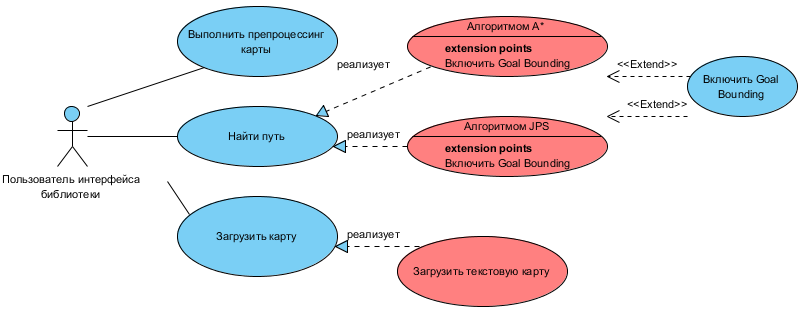
\includegraphics[width=1\linewidth]{path_finding_use_case.png}
\end{frame}

\begin{frame}{Проектирование}{Диаграмма классов}
\centering
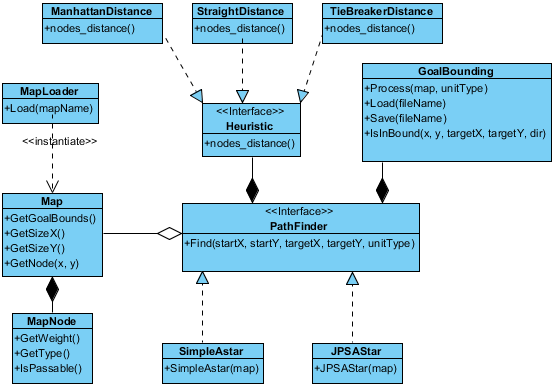
\includegraphics[width=1\linewidth]{path_finding_classes.png}
\end{frame}

\begin{frame}{Алгоритм A*}{}
A* является вариацией алгоритма Дейкстры и использует эвристическую функция для ускорения работы. 

\vspace{\baselineskip}

Алгоритм минимизирует функцию точки $ f(n) = g(n) + h(n) $, где $g(n)$ -- стоимость пути до точки, а $h(n)$ -- эвристическая оценка стоимости прохождения до конца пути.

\vspace{\baselineskip}

Алгоритм останавливается когда точкой с наименьшей стоимостью является конечная точка, или список для рассмотрения пуст.
\end{frame}

\begin{frame}{Алгоритм A*}{Визуализация}
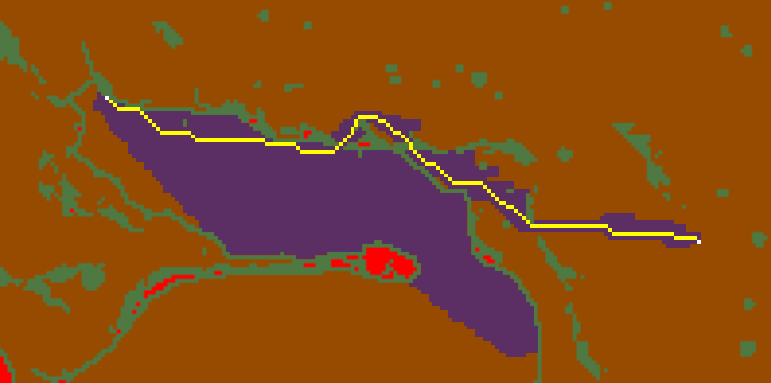
\includegraphics[width=1\linewidth]{a_star_on_map.png}

Жёлтым обозначен путь, фиолетовым -- точки добавленные в открытый список.
\end{frame}

\begin{frame}{Алгоритм A*}{Результаты на карте AR0011SR (512x512)}

\begin{tabular*}{\textwidth}{c@{}c@{}}
\begin{minipage}{\dimexpr0.65\textwidth-2\tabcolsep}
\centering
\begin{tikzpicture}[scale=0.8]
    \begin{axis}[
		name=plot1,
		xlabel={Стоимость пути},
		ylabel={миллисекунды},
		legend pos=north west]
		\addplot[smooth,mark=*,black] plot coordinates {
	(0,0.450337827586206897 )
	(30,0.473905788888888889)
	(60,0.526151056179775281)
	(90,0.603534767676767677)
	(120,0.859617405063291139)
	(150,1.0536403333333333  )
	(180,1.3990839574468085  )
	(210,2.2270172111111111  )
	(240,2.3663113736263736  )
	(270,3.01304575          )
	(300,3.848451175         )
	(330,4.4758353296703297  )
	(360,5.6996502413793103  )
	(390,6.27858416          )
	(420,7.6057240178571429  )
	(450,8.6096742142857143  )
		};
		\legend{A*}
	\end{axis}
\end{tikzpicture}
\end{minipage}
&
\begin{minipage}[t]{\dimexpr0.35\textwidth-2\tabcolsep}
\hfill
    \begin{tabular}{|l|c|}
    \hline
    Длина & мс \\
    \hline
    0 & 0.45 мс   \\
    \hline
    50 & 0.52 мс \\
    \hline
    100 & 0.74 мс \\
    \hline
    150 & 1.12 мс \\
    \hline
    200 & 2.15 мс \\
    \hline
    250 & 2.69 мс \\
    \hline
    300 & 3.90 мс \\
    \hline
    350 & 5.60 мс \\
    \hline
    400 & 7.03 мс \\
    \hline
    450 & 8.60 мс \\
    \hline
    \end{tabular}
\end{minipage}
\end{tabular*}%

\vspace{0.5\baselineskip}

По результатам видно, что время выполнения одного поиска пути для A* находится от 0.5 до 9 миллисекунд. Такое время слишком велико для игр.

\end{frame}

\begin{frame}{Алгоритм JPS}{}

Jump Point Search -- эффективная техника для нахождения и отброса симметричных путей, основана на алгоритме A*. Избавляет A* от необходимости рассматривать симметричные пути и точки, которые не могут входить в оптимальный маршрут.

\addtikz{Симметричные пути}{symmetric_paths}{0.7}
{
	\mybox[x=1,y=1,color=green]
	\mybox[x=4,y=4,color=green]
	
	\mygrid[width=6, height=6]
	
	\myarrow[startx=1,starty=1,endx=1,endy=2,color=blue]
	\myarrow[startx=1,starty=2,endx=1,endy=3,color=blue]
	\myarrow[startx=1,starty=3,endx=1,endy=4,color=blue]
	\myarrow[startx=1,starty=4,endx=2,endy=4,color=blue]
	\myarrow[startx=2,starty=4,endx=3,endy=4,color=blue]
	\myarrow[startx=3,starty=4,endx=4,endy=4,color=blue]
	
	\myarrow[startx=4,starty=1,endx=4,endy=2,color=orange]
	\myarrow[startx=4,starty=2,endx=4,endy=3,color=orange]
	\myarrow[startx=4,starty=3,endx=4,endy=4,color=orange]
	\myarrow[startx=1,starty=1,endx=2,endy=1,color=orange]
	\myarrow[startx=2,starty=1,endx=3,endy=1,color=orange]
	\myarrow[startx=3,starty=1,endx=4,endy=1,color=orange]
	
	\myarrow[startx=1,starty=2,endx=2,endy=2,color=red]
	\myarrow[startx=2,starty=2,endx=3,endy=2,color=red]
	\myarrow[startx=3,starty=2,endx=4,endy=2,color=red]
	
	\myarrow[startx=1,starty=3,endx=2,endy=3,color=black]
	\myarrow[startx=2,starty=3,endx=3,endy=3,color=black]
	\myarrow[startx=3,starty=3,endx=4,endy=3,color=black]
}

\end{frame}

\begin{frame}{Алгоритм JPS}{Результаты на карте AR0011SR (512x512)}

\begin{tabular*}{\textwidth}{c@{}c@{}}
\begin{minipage}{\dimexpr0.60\textwidth-2\tabcolsep}
\centering
\begin{tikzpicture}[scale=0.75]
    \begin{axis}[
		name=plot1,
		xlabel={Стоимость пути},
		ylabel={микросекунды},
		ytick scale label code/.code={},
		scaled y ticks=base 10:3,
		legend pos=north west]
		\addplot[smooth,mark=*,black] plot coordinates {
			(0,0.012311942857142857  )
			(30,0.015875864197530864 )
			(60,0.01732458904109589  )
			(90,0.01950175           )
			(120,0.023366141025641026)
			(150,0.025258567567567568)
			(180,0.027953415584415584)
			(210,0.029131767123287671)
			(240,0.036167641975308642)
			(270,0.038806767123287671)
			(300,0.04332785          )
			(330,0.048559086956521739)
			(360,0.049925911392405063)
			(390,0.054420759036144578)
			(420,0.0565024           )
			(450,0.050475512195121951)
			(480,0.07050855)
		};
		\legend{JPS}
	\end{axis}
\end{tikzpicture}
\end{minipage}
&
\begin{minipage}[t]{\dimexpr0.4\textwidth-2\tabcolsep}
\hfill
    \begin{tabular}{|l|c|}
    \hline
    Длина & мс \\
    \hline
    0 & 0.060 мс \\
    \hline
    50 & 0.0895 мс \\
    \hline
    100 & 0.110 мс \\
    \hline
    150 & 0.145 мс \\
    \hline
    200 & 0.160 мс \\
    \hline
    250 & 0.232 мс \\
    \hline
    300 & 0.277 мс \\
    \hline
    350 & 0.379 мс \\
    \hline
    400 & 0.536 мс \\
    \hline
    450 & 0.668 мс \\
    \hline
    \end{tabular}
\end{minipage}
\end{tabular*}%

\vspace{0.5\baselineskip}

По результатам JPS на порядок быстрее A*.

\end{frame}

\begin{frame}{Алгоритм Gaol Bounding}{}

Goal Bounding -- техника отброса заранее неподходящих направлений, которая позволяет значительно ускорить поиск пути. Включает оффлайн и онлайн этапы. 

\begin{itemize}
    \item Оффлайн этап -- обработка карты с целью найти и сохранить для каждой точки направления с кратчайшими путями;
    \item Онлайн этап -- проверка может ли являться путь в выдранном направлении кратчайшим.
\end{itemize}

Является крайне затратным по времени для карт размером более 512 на 512, однако очень хорошо поддаётся параллелизации.

\end{frame}

\begin{frame}{Алгоритм Gaol Bounding}{Визуализация}

\begin{figure}
    \centering
    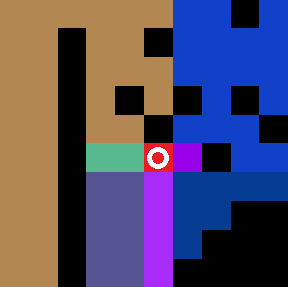
\includegraphics[width=0.5\linewidth]{goal_bound_visualisation.png}
\end{figure}


Каждый цвет показывает в каком направлении следует идти что бы дойти до покрашенной точки по кратчайшему пути.
\end{frame}

\begin{frame}{Общее сравнение}{}

\hspace{-1.5em}
	\begin{tabular}{|l|c|c|c|c|c|c|c|}
		\hline
Cost& A* & A*GB& от A* &JPS& от A*&JPS+GB& от A* \\
\hline 	
0	& 0,36	& 0,16	& 43,80\%	& 0,024	& 06,50\%	& 0,005 & 01,28\% \\
\hline
60	& 0,48	& 0,28	& 58,10\%	& 0,065	& 13,33\%	& 0,012 & 02,45\% \\
\hline
120	& 0,72	& 0,33	& 46,63\%	& 0,103	& 14,27\%	& 0,016 & 02,27\% \\
\hline
180	& 1,16	& 0,39	& 33,87\%	& 0,150	& 12,84\%	& 0,021 & 01,76\% \\
\hline
240	& 1,78	& 0,46	& 25,93\%	& 0,205	& 11,48\%	& 0,025 & 01,38\% \\
\hline
300	& 2,63	& 0,53	& 20,28\%	& 0,275	& 10,43\%	& 0,029 & 01,12\% \\
\hline
360	& 3,74	& 0,58	& 15,53\%	& 0,358	& 09,57\%	& 0,033 & 00,89\% \\
\hline
420	& 4,85	& 0,54	& 11,31\%	& 0,481	& 09,90\%	& 0,039 & 00,80\% \\
\hline
480	& 4,97	& 0,41	& 08,38\%	& 0,569	& 11,44\%	& 0,040 & 00,81\% \\
\hline
540	& 5,32	& 0,45	& 08,52\%	& 0,828	& 15,56\%	& 0,050 & 00,93\% \\
\hline
	\end{tabular}

\vspace{0.5\baselineskip}

Алгоритм Goal Bounding ускоряет A* в 2 -- 10 раз, а JPS в 5 -- 15 раз. JPS с Goal Bounding быстрее обычного A* в 40 -- 100 раз.

\end{frame}

\begin{frame}{Выводы}{}

\setlength\parindent{24pt}

Во время выполнения работы были проанализированы и реализованы алгоритмы нахождения кратчайшего пути A*, JPS и Goal Bounding. Была спроектирована, реализована и протестирована библиотека включающая указанные алгоритмы.

Из рассмотренных алгоритмов самым быстрым является JPS с Goal Bounding, однако при этом он является самым не универсальным. 

Для карт с одинаковой стоимостью прохождения по клеткам наилучшим выбором оказался JPS. 

Для карт с разной стоимостью прохождения по клеткам наилучшим будет алгоритм A* с или без Goal Bounding.

\end{frame}

\end{document}


